\documentclass[11pt]{article}

% --- arXiv-ready preamble -------------------------------------------------
\usepackage[utf8]{inputenc}
\usepackage[T1]{fontenc}
\usepackage{lmodern}
\usepackage{amsmath,amssymb}
\usepackage{graphicx}
\usepackage{booktabs}
\usepackage{microtype}
\usepackage[margin=1in]{geometry}
\usepackage[hidelinks]{hyperref}

\newcommand{\sph}{\operatorname{sph}}
\newcommand{\atantwo}{\operatorname{atan2}}
\newcommand{\slotf}{\operatorname{slot}}
\renewcommand{\deg}{^{\circ}}  % \deg is a LaTeX kernel command; redefine as a degree symbol (used only in math mode)

\title{A Spherical-Coordinate Chain Representation of Text\\[2pt]
\large A Self-Describing, Reversible Encoding of Symbol Sequences in 3D}

\author{Author name(s) \\ Affiliation \\ \texttt{email@example.com}}
\date{July 2026 \\[4pt] \small Working preprint --- not yet submitted}

\begin{document}
\maketitle

\begin{abstract}
We present a method for representing text---or any sequence over a fixed symbol
alphabet---as a chain of unit vectors in three-dimensional space, expressed in spherical
coordinates. Each symbol maps to one step vector $(r,\alpha,\varphi)$: the azimuth
$\varphi$ encodes the symbol's identity through a $90$-position dial spaced at $4\deg$
(printable ASCII with its five least-frequent characters removed), while the elevation
$\alpha$ accumulates by a fixed increment per symbol, so that successive steps trace an
ascending spiral. Steps are joined tip-to-tail in a translational frame whose axes remain
parallel to the global frame, making both angles absolute. The representation is
\emph{self-describing}: each step vector independently reports its position in the sequence
(from $\alpha$) and its symbol (from $\varphi$), so decoding requires no external state. We
show the encoding is exactly reversible for $0\deg<\alpha<90\deg$, recovering the original
sequence from node coordinates alone; beyond this range steps alias and reversibility
fails, which bounds the usable length. We emphasize that this is a geometric representation
and visualization, \emph{not} a compression scheme---stored as coordinates the chain
expands rather than shrinks. The construction adapts internal-coordinate (Z-matrix) and
chain-code ideas from chemistry and image processing to text, and induces a geometric
fingerprint in which shared prefixes trace coincident curves.
\end{abstract}

% =========================================================================
\section{Introduction}

Text is almost always stored and manipulated as a linear stream of symbols. Yet much of the
structure in a sequence---repetition, shared prefixes, the boundary between one token and
the next---is easier to see than to read. This paper asks a deliberately simple question:
what happens if we turn a symbol sequence into a shape? We map each symbol to a short step
in three-dimensional space and lay the steps tip-to-tail, so that a string becomes a path
and a vocabulary becomes a family of paths.

The construction is spare. Each symbol is one unit step written in spherical coordinates
$(r,\alpha,\varphi)$. The azimuth $\varphi$---the compass bearing of the step in the
horizontal plane---encodes \emph{which} symbol it is, through a $90$-position dial spaced at
$4\deg$ (the printable ASCII set with its five least-frequent characters removed). The
elevation $\alpha$---how far the step tilts above the horizontal---encodes \emph{where} the
symbol sits in the sequence: $\alpha$ accumulates by a fixed increment per step, so the path
climbs as it advances. The radius $r$ is constant and carries no information. Steps are
joined in a frame whose axes stay parallel to the global frame, so both angles are absolute
rather than relative to the preceding step.

Two properties follow, and we prove both. First, the encoding is \emph{self-describing}:
because $\varphi$ fixes the symbol and $\alpha$ fixes the position, every step vector, taken
in isolation, reports both what it is and where it belongs---decoding needs no external
index or state. Second, it is \emph{reversible}: within the regime $0\deg<\alpha<90\deg$ the
original sequence is recovered exactly from the node coordinates alone, with no access to
the source text. We also characterize where reversibility breaks: at $\alpha=90\deg$ a step
points straight up and its azimuth is lost, and beyond $90\deg$ steps alias with their
reflections; together these bound the usable length to about $90\deg/\Delta$ symbols.

We are equally explicit about what the method is \emph{not}. It is a representation and a
visualization, not a compression scheme. A symbol carries about $\log_2 90 \approx 6.5$
bits, whereas a coordinate triple carries more, so storing the chain as geometry expands the
data rather than shrinking it; the right way to store a chain is to keep the symbol sequence
and redraw the geometry on demand. We make this precise in Section~\ref{sec:compression},
because the geometric framing invites the opposite---and incorrect---intuition.

The payoff of the geometric view is legibility. A small change to the encoding---accumulating
$\alpha$ from the start of each \emph{word} rather than the start of the text---makes a
word's shape independent of where the word appears. Identical words then trace identical
shapes, and words that share a spelling prefix share the initial segment of their path.
Rendered together, a vocabulary fans out from the origin into a three-dimensional
\emph{prefix tree} (Figure~\ref{fig:prefixtree}): common beginnings bundle near the root and
branch where spellings diverge, and repeated words coincide exactly. The structure is not
imposed; it is a direct consequence of a deterministic, per-symbol map.

\begin{figure}[t]
  \centering
  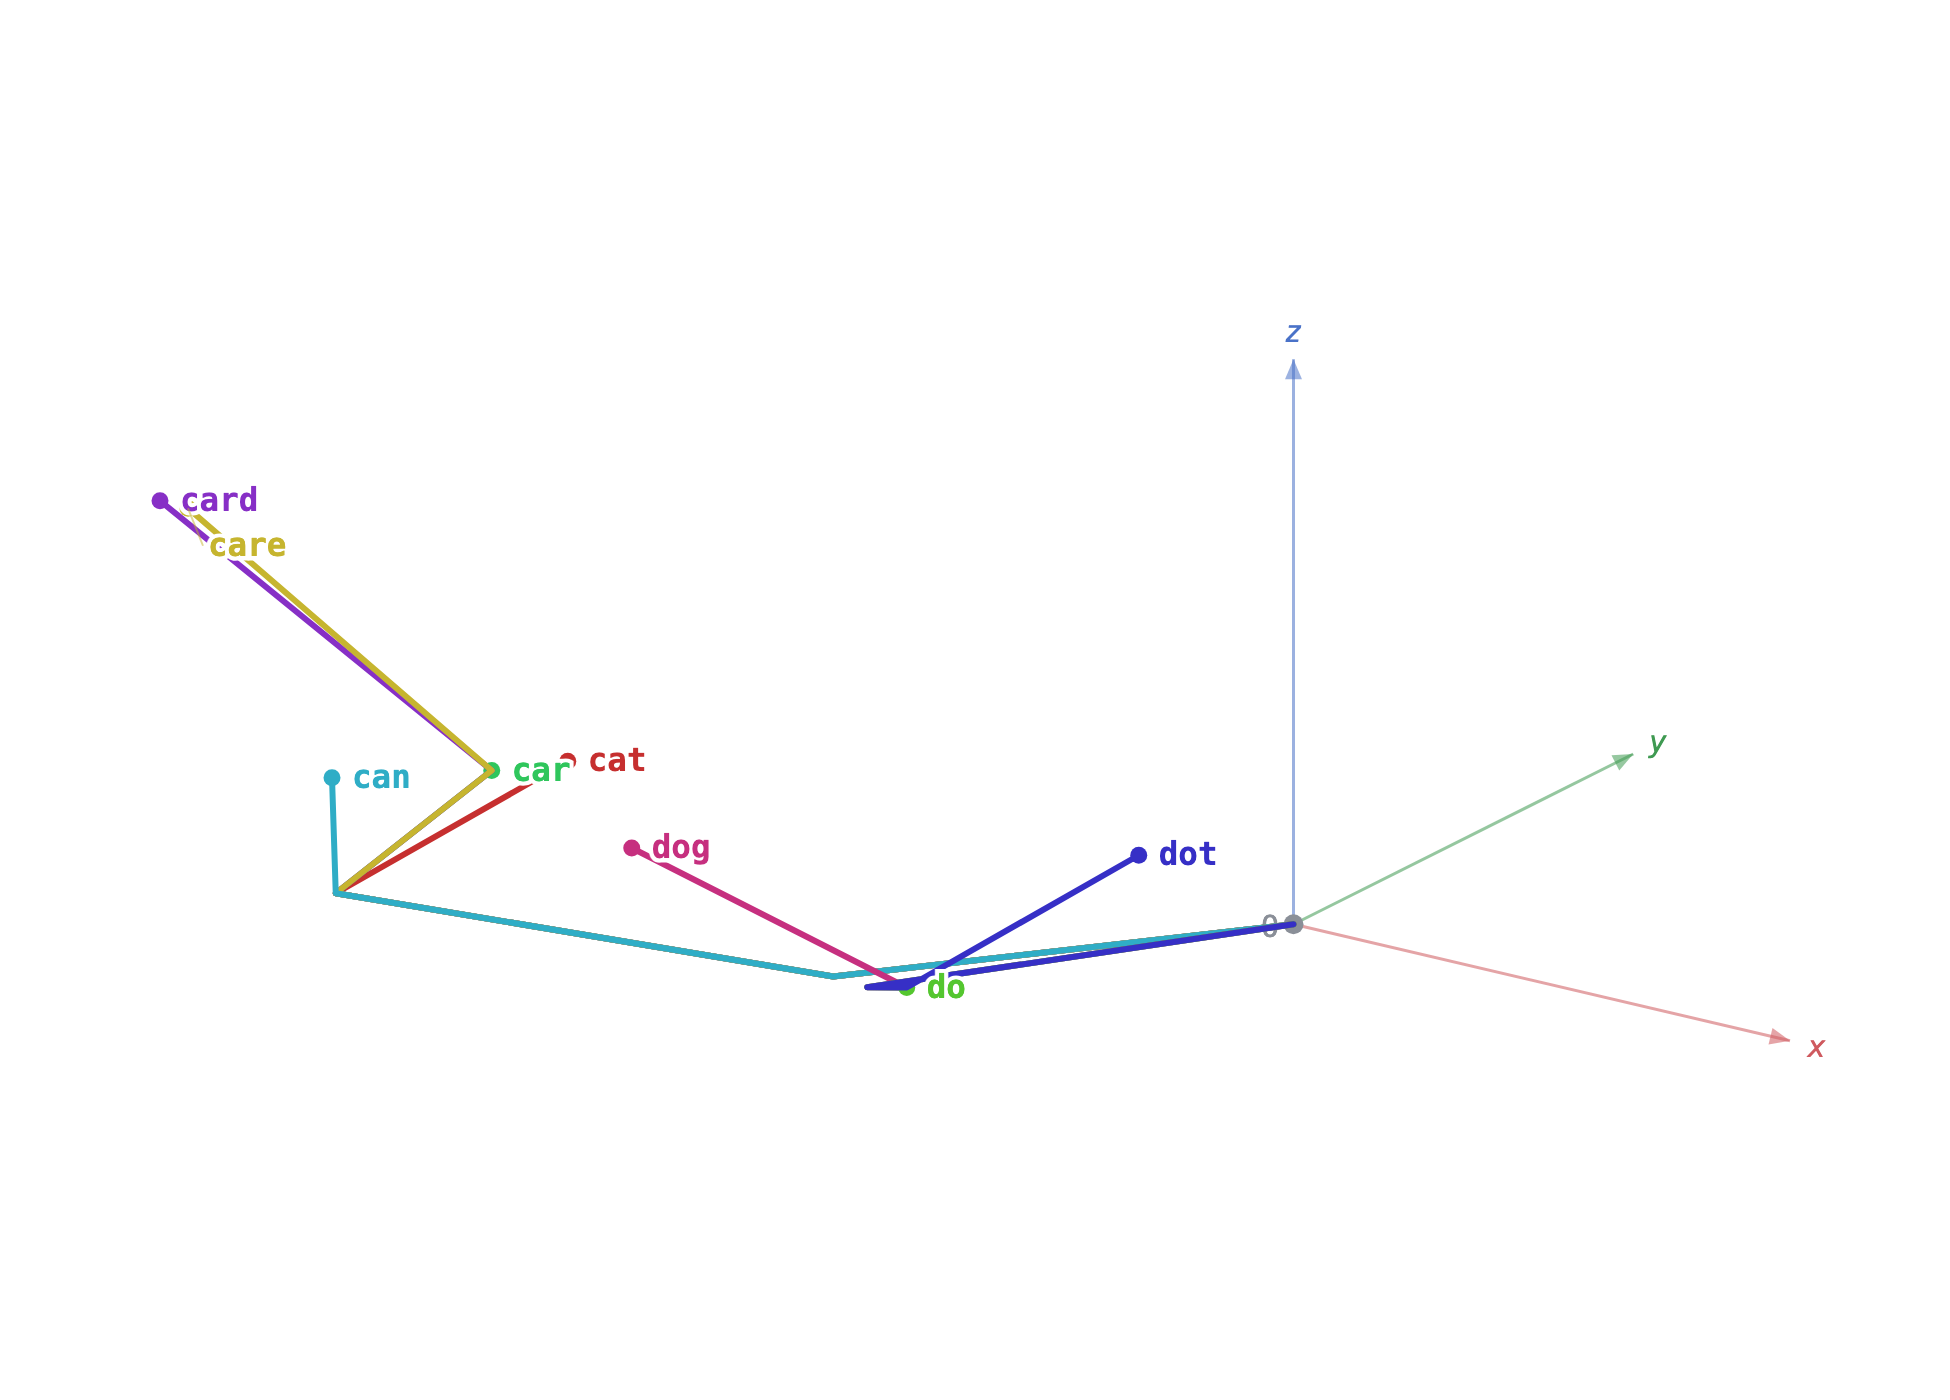
\includegraphics[width=0.92\linewidth]{figures/prefix-tree.png}
  \caption{A vocabulary as a three-dimensional prefix tree. Each word is a chain of unit
  steps from a common origin under the word-local encoding (azimuth $=$ character, elevation
  $=$ within-word position, $10\deg$ step). Words sharing a spelling prefix share the initial
  segment of their path and branch where they differ; identical words coincide. Vocabulary:
  \{cat, car, card, care, can, dog, do, dot\}.}
  \label{fig:prefixtree}
\end{figure}

\paragraph{Contributions.} We (i) define a spherical-coordinate chain encoding of symbol
sequences in which azimuth carries identity and cumulative elevation carries position,
making each step vector self-describing; (ii) prove exact reversibility within
$0\deg<\alpha<90\deg$ and characterize the failure modes and resulting length bound; (iii)
give an information-theoretic account of why the representation does not compress; (iv)
introduce a word-local variant whose shapes are position-invariant, so a vocabulary renders
as a 3D prefix tree with identical words coinciding and shared prefixes shared; and (v)
provide an interactive tool that encodes, decodes-and-verifies, and renders all of the
above.

\paragraph{Relation to prior work.} The construction adapts two mature ideas to a new use.
Internal-coordinate (Z-matrix) representations in chemistry place each atom relative to its
predecessors by a length and two angles; Freeman chain codes in image processing encode a
curve as a sequence of quantized step directions. We apply the same relative-step idea to
text, binding symbol identity to direction, and relate the resulting word shapes to the
``word as trajectory'' view familiar from word-gesture keyboards. Section~\ref{sec:related}
develops these connections; here we note only that, to our knowledge, the use of an
internal-coordinate chain as a reversible, self-describing representation of text---and the
prefix-tree visualization it induces---has not been described.

% =========================================================================
\section{Encoding}\label{sec:encoding}

We encode a sequence of symbols $s_1 s_2 \dots s_n$. Each symbol contributes one step; the
$k$-th step is a vector $v_k$ written in spherical coordinates $(r,\alpha,\varphi)$ and
interpreted in a frame attached to the previous node (Section~\ref{sec:frame}). The three
coordinates play distinct roles: $\varphi$ carries the symbol's identity, $\alpha$ carries
its position in the sequence, and $r$ is a fixed scale.

\subsection{Azimuth $\varphi$ --- symbol identity}

We fix an alphabet of $90$ symbols: the $95$ printable ASCII characters (0x20--0x7E) with
the five least-frequent removed (\verb.` ^ ~ { }.). The remaining characters, in ASCII
order, occupy slots $0$--$89$, and a symbol's azimuth is
\[
  \varphi(s) = \slotf(s)\times 4\deg, \qquad \slotf(s)\in\{0,\dots,89\}, \qquad
  \varphi\in\{0\deg,4\deg,\dots,356\deg\}.
\]
Choosing $90$ makes $360\deg$ divide evenly, so every azimuth is an integer multiple of
$4\deg$. The empty symbol occupies no slot; it is represented by a zero-length step ($r=0$),
read back as ``no content.'' Because ASCII orders characters contiguously, like symbols land
in contiguous arcs of the dial (digits at $64\deg$--$100\deg$, uppercase at
$132\deg$--$232\deg$, lowercase at $252\deg$--$352\deg$).

\subsection{Elevation $\alpha$ --- sequence position}

The elevation accumulates by a fixed increment $\Delta$ per symbol,
\[
  \alpha_k = k\cdot\Delta, \qquad \text{with default } \Delta = 10\deg.
\]
Because $\alpha$ advances monotonically, position is recorded by the geometry itself: the
$k$-th step tilts higher than the $(k{-}1)$-th, and $k = \alpha_k/\Delta$ recovers the index.
No separate position field is stored. Section~\ref{sec:reversibility} shows this is exactly
what makes the code self-describing, and what bounds its length.

\subsection{Radius $r$}

The radius is constant, $r=1$, and carries no information; it sets the step length. (A
variant that lets $r$ grow with $k$ is possible but unused here.)

\subsection{Step vector, frame, and chain}\label{sec:frame}

We measure $\alpha$ from the horizontal ($xy$) plane---an elevation, not a zenith angle---so
that small angles give near-horizontal steps with a large horizontal projection. The
Cartesian step is
\[
  \sph(r,\alpha,\varphi) = \bigl(r\cos\alpha\cos\varphi,\; r\cos\alpha\sin\varphi,\;
  r\sin\alpha\bigr),
\]
with horizontal component $r\cos\alpha$ and vertical component $r\sin\alpha$. Steps are laid
tip-to-tail from the origin $N_0 = O$:
\[
  N_k = N_{k-1} + R_{k-1}\cdot \sph(v_k).
\]
We use the \emph{translational frame}: every node frame keeps its axes parallel to the global
frame ($R_k = I$), so the two angles are absolute---$\varphi$ from the global $+x$ axis,
$\alpha$ from the global horizontal---and $R_{k-1}\cdot\sph(v_k) = \sph(v_k)$. This is the
property that lets a single step be decoded in isolation (Section~\ref{sec:selfdesc}). An
alternative co-moving frame that rotates $+z$ onto the incoming direction makes $\alpha$ a
bend angle relative to the previous step; it is more expressive but unnecessary here, since
position is already carried by cumulative $\alpha$.

As a worked example, \texttt{cat} at $\Delta=10\deg$ gives slots $(65,63,82)$, azimuths
$(260\deg,252\deg,328\deg)$, elevations $(10\deg,20\deg,30\deg)$, and nodes
$N_1=(-0.171,-0.970,0.174)$, $N_2=(-0.461,-1.864,0.516)$, $N_3=(0.273,-2.322,1.016)$.

% =========================================================================
\section{Self-description and decoding}\label{sec:selfdesc}

\subsection{The self-describing property}\label{sec:selfprop}

Call an encoding \emph{self-describing} if each step vector, examined on its own---without
its neighbours and without a stored index---determines both the symbol it carries and its
position in the sequence. The construction of Section~\ref{sec:encoding} has this property on
the reversible regime.

Under the translational frame a step is $v_k = \sph(1,\alpha_k,\varphi_k)$ in global
coordinates, with $\alpha_k = k\cdot\Delta$ and $\varphi_k = \slotf(s_k)\cdot 4\deg$. From the
components of $v_k$ alone,
\[
  r = |v_k|, \qquad \alpha = \arcsin(v_{k,z}/r), \qquad \varphi = \atantwo(v_{k,y},v_{k,x}),
\]
and therefore $k = \alpha/\Delta$ (position) and $\slotf = \operatorname{round}(\varphi/4\deg)$
(symbol). No neighbouring step, running index, or table of offsets is consulted: a lone
vector reports what it is through its bearing and where it belongs through its tilt. This
follows directly from the two design choices of Section~\ref{sec:encoding}---absolute angles
and cumulative elevation. In a co-moving frame the elevation would be a bend relative to the
previous step, and a single vector could no longer name its absolute position; the property
would be lost.

\subsection{Decoding a chain}

To decode we are given the node coordinates $N_0,N_1,\dots,N_n$---pure geometry, with no
access to the source text---together with the protocol (the increment $\Delta$, the
$90$-symbol dial, the translational frame). For each step we recover the displacement and
read off its symbol:
\begin{verbatim}
decode(N_0 ... N_n):
  for k = 1 ... n:
      v = N_k - N_{k-1}          # translational frame: v is the global step
      r = |v|
      if r ~= 0:  emit null (empty symbol); continue
      alpha = arcsin(v_z / r)
      phi   = atan2(v_y, v_x)  (mod 360 deg)
      slot  = round(phi / 4 deg) mod 90
      emit CHARSET[slot]
  return the emitted sequence
\end{verbatim}
Because the chain already presents its steps in order, the index $k$ obtained from $\alpha$
is redundant with a step's ordinal position. We keep it deliberately: whenever
$\operatorname{round}(\alpha/\Delta)$ disagrees with a step's place in the chain, the
discrepancy flags corruption or a frame error. Self-description thus doubles as a built-in
checksum.

\subsection{A fragment locates itself}\label{sec:fragment}

Self-description has a consequence the whole-chain view obscures: one need not have the whole
chain to read part of it. Any single step---equivalently, any adjacent pair of nodes---yields
both its character and its absolute index. A fragment cut from the middle of a chain
therefore self-locates: it announces which symbols it holds and where, in the original
sequence, they sat, with no header and no surrounding context. We exploit this for the
fingerprints of Section~\ref{sec:fingerprints}, and it fails exactly where reversibility
fails, at $\alpha\ge 90\deg$.

\subsection{Correctness}

Decoding is exact precisely when the map $(\alpha,\varphi)\mapsto\text{direction}$ is
injective over the elevations used. It is injective for $0\deg<\alpha<90\deg$: the elevation
is recovered without ambiguity because $\sin$ is strictly monotone there, and the azimuth is
then recovered because $\cos\alpha>0$. Section~\ref{sec:reversibility} proves this, exhibits
the two ways it breaks---a vertical step at $\alpha=90\deg$ and reflection aliasing beyond
$90\deg$---and separates what this costs.

\subsection{Robustness of decoding}

Decoding needs two things from each step---its symbol and its position---and the geometry
supplies each in more than one way. The redundancy makes the decoder resistant to
disordering, to local corruption, and to silent failure.

\paragraph{Position has three independent sources.} The symbol is read from the azimuth
alone, but a step's position $k$ can be recovered three ways: (a) from its ordinal place in
the node list; (b) from its own elevation, $k=\alpha/\Delta$, since a single step in the
self-describing regime reports its index (Section~\ref{sec:selfprop}); and (c) by sorting the
nodes on height, since $z$ increases monotonically while $\alpha<180\deg$. Any one suffices.
The last deserves stating plainly: even a bag of nodes with the order discarded decodes,
because sorting on $z$ reconstructs the order first---encoding \texttt{spiral}, shuffling its
seven nodes, sorting by height, and decoding returns \texttt{spiral} exactly. When more than
one source is available they cross-check: if the index from $\alpha$ disagrees with the
ordinal place, the discrepancy signals corruption. The self-description of
Section~\ref{sec:selfprop} thus doubles as a built-in integrity check, at no cost.

\paragraph{Decoding is local.} Each step is recovered from just its two endpoints, $N_{k-1}$
and $N_k$, so a corrupted node damages only the two steps that touch it; the error does not
propagate down the chain, unlike a sequential code in which one early error corrupts
everything after.

\paragraph{Failures are detected, not silent.} Where a character cannot be recovered, the
decoder says so. A vertical step ($\cos\alpha_k\approx 0$) has no azimuth: it emits a marked
gap rather than a wrong guess, and knows exactly which position is affected. A zero-length
step ($r\approx 0$) decodes to the empty symbol. Near a vertical the horizontal projection is
small and the azimuth is noise-sensitive, so such steps can be flagged low-confidence instead
of reported as a spurious character.

\paragraph{The sources degrade gracefully with elevation.} For $0\deg<\alpha<90\deg$ all
three position sources hold, giving maximum redundancy and letting any fragment self-locate
(Section~\ref{sec:fragment}). For $90\deg<\alpha<180\deg$ the elevation folds (b fails), but
height is still monotonic (c) and the list order (a) is intact, so full-chain decoding is
unaffected. Beyond $180\deg$ height is no longer monotonic (c fails) and only the given order
remains. Reversibility rests, in the last resort, on the ordering of the nodes---which in the
common regime the geometry reconstructs for free.

% =========================================================================
\section{Reversibility}\label{sec:reversibility}

Whether the code is reversible turns on how a step vector determines its character, and that
determination changes at $\alpha=90\deg$. We first locate the difficulty in the isolated
vector, then show that the chain removes it.

\subsection{The ambiguity is in the isolated coordinate}

A step is decoded by reading its azimuth, $\varphi=\atantwo(v_y,v_x)$. This returns the
character's azimuth only while the horizontal projection points along $\varphi$---that is,
while $\cos\alpha>0$. Two identities of the unit direction
$d(\alpha,\varphi)=(\cos\alpha\cos\varphi,\cos\alpha\sin\varphi,\sin\alpha)$ govern the rest:
\[
  d(\alpha,\varphi) = d(\alpha+360\deg,\varphi) \quad\text{(periodicity)}, \qquad
  d(\alpha,\varphi) = d(180\deg-\alpha,\varphi+180\deg) \quad\text{(reflection)}.
\]
The reflection is the crux. Past vertical ($\alpha>90\deg$) the sign of $\cos\alpha$ reverses,
so the horizontal projection points along $\varphi+180\deg$ and the azimuth reads as a
\emph{different} character. Concretely, a step for \texttt{c} ($\varphi=260\deg$) at
$\alpha=100\deg$ is the identical vector to a step for \texttt{4} ($\varphi=80\deg$) at
$\alpha=80\deg$: both are $(0.030,0.171,0.985)$. Converting that vector back to spherical
coordinates gives the single canonical reading $(r{=}1,\alpha{=}80\deg,\varphi{=}80\deg)$---the
\texttt{4} reading; the intended $(\alpha{=}100\deg,\varphi{=}260\deg)$ has folded onto its
reflection. So the map $(\alpha,\varphi)\to\text{direction}$ is not injective once $\alpha$
passes $90\deg$, and it is singular at the pole $\alpha=90\deg$ (the point $(0,0,1)$), where
no azimuth exists at all. Both are defects of the isolated spherical triple
(Figure~\ref{fig:reflection}).

\begin{figure}[t]
  \centering
  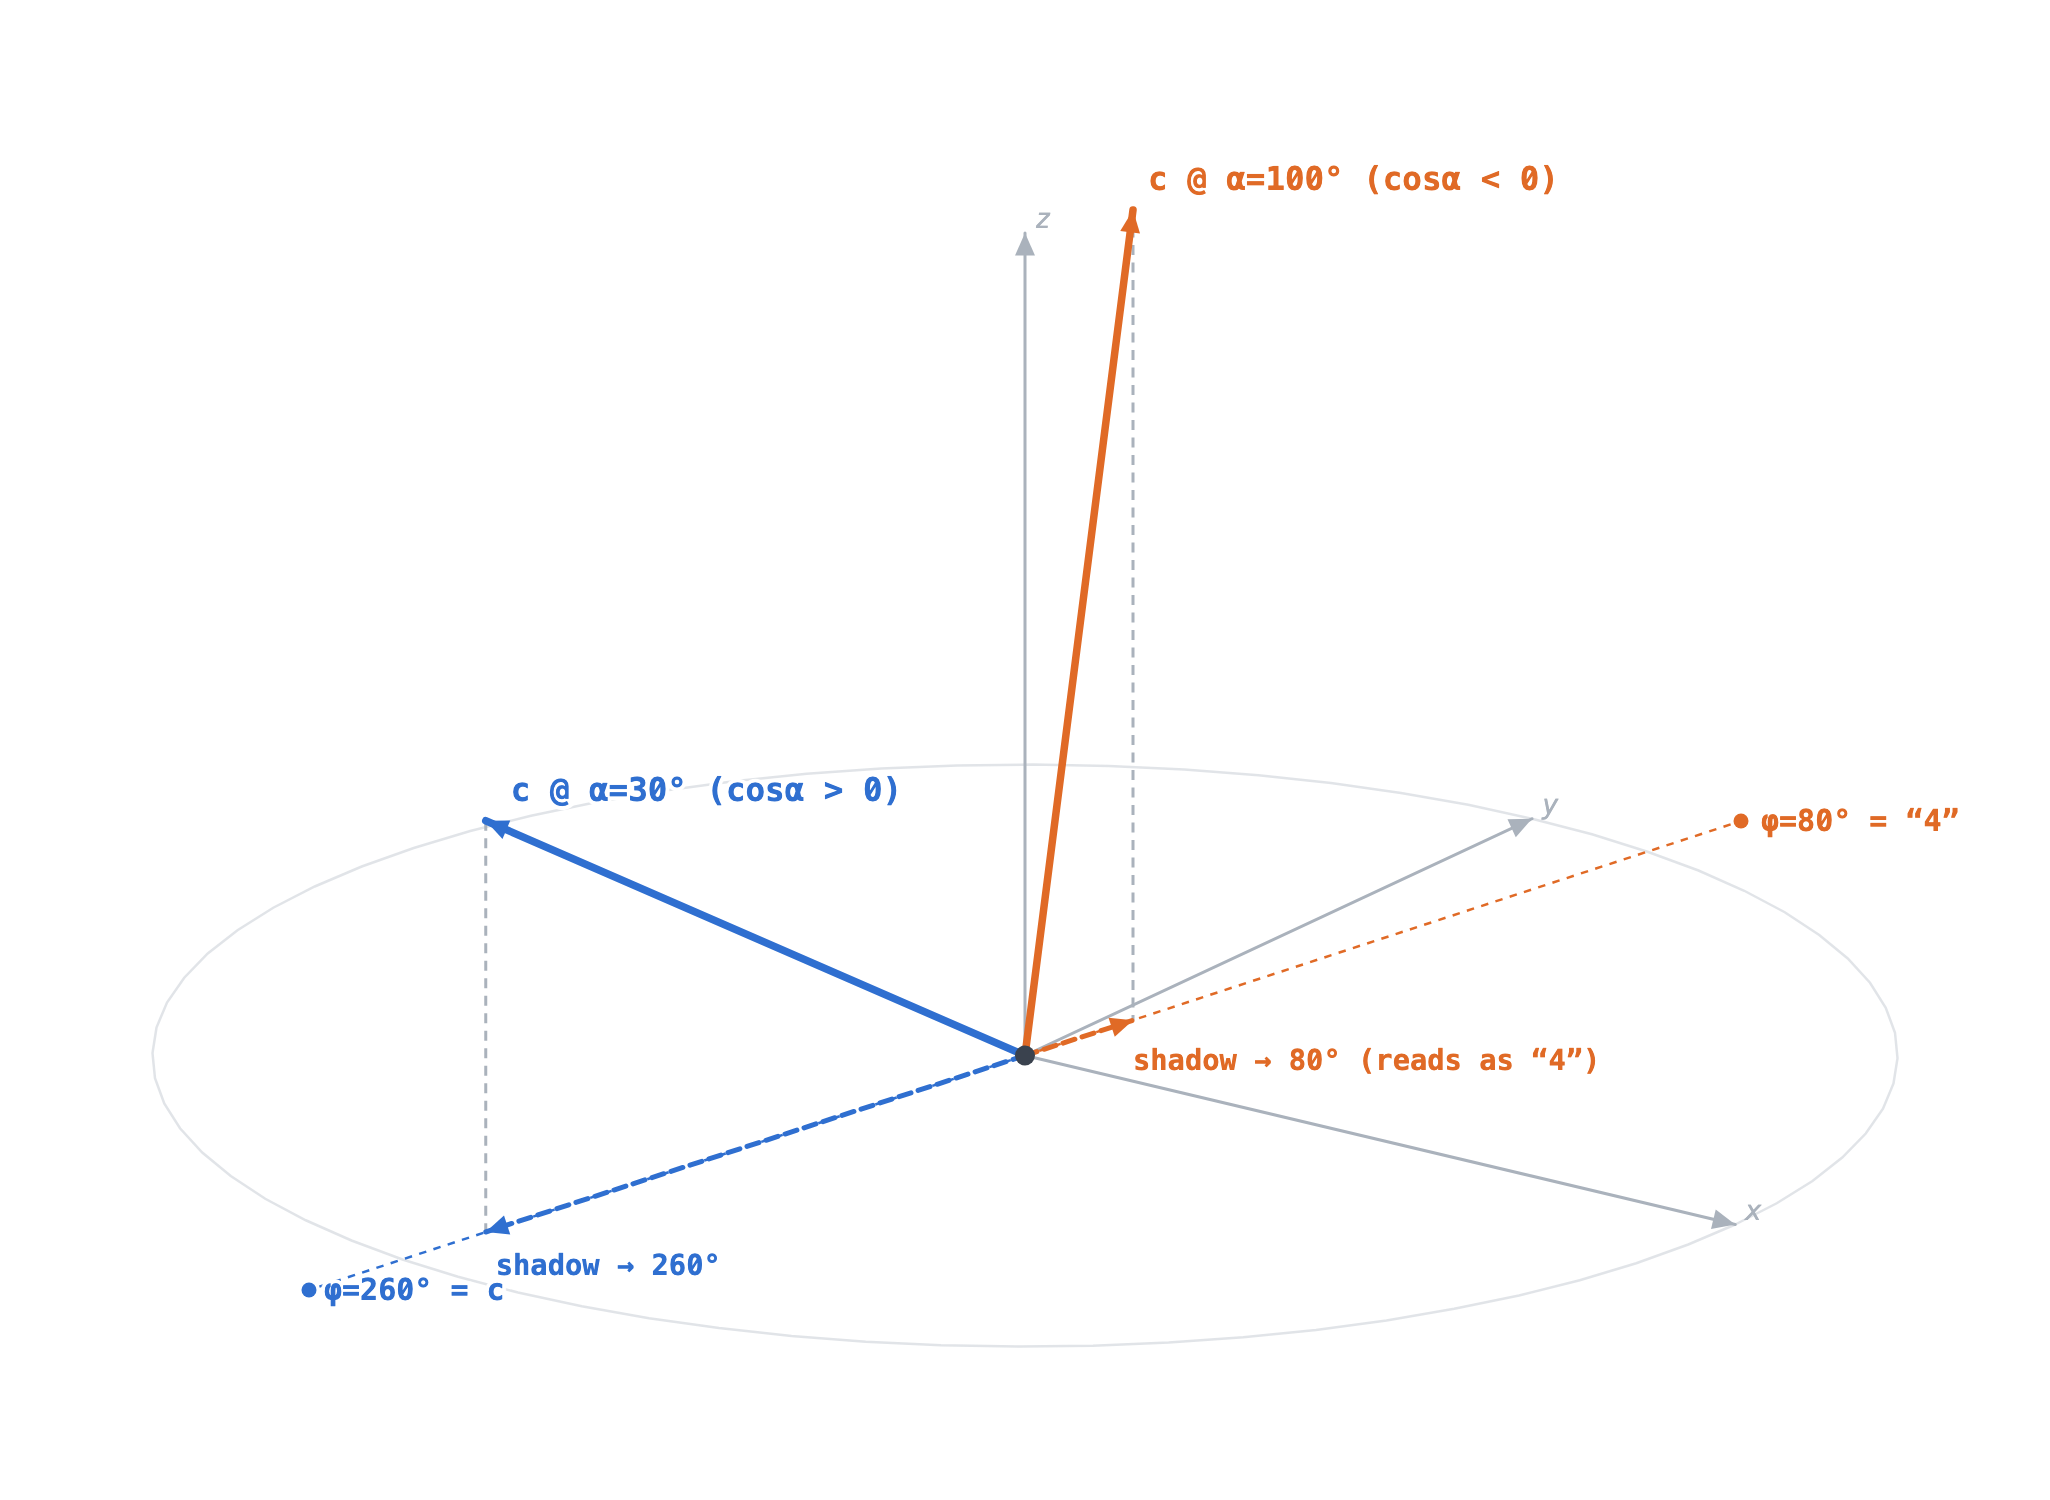
\includegraphics[width=0.9\linewidth]{figures/reflection-flip.png}
  \caption{Why reversibility breaks past $\alpha=90\deg$. The same character \texttt{c}
  (azimuth $\varphi=260\deg$) drawn at $\alpha=30\deg$ (blue) and $\alpha=100\deg$ (orange),
  with its ground shadow. A step's shadow points along $\varphi$ only while $\cos\alpha>0$;
  once $\alpha$ passes vertical, $\cos\alpha<0$ and the shadow flips by $180\deg$---here to
  $80\deg$, the bearing of the character \texttt{4}. Knowing $\alpha$ undoes the flip; at
  exactly $\alpha=90\deg$ the shadow vanishes and the azimuth is lost.}
  \label{fig:reflection}
\end{figure}

\subsection{The chain carries the missing elevation}

The encoding does not store isolated vectors; it stores an ordered chain. Step $k$ is the
displacement $v = N_k - N_{k-1}$, and the chain gives its ordinal position $k$ directly---hence
its true elevation $\alpha_k = k\cdot\Delta$, even when $\alpha_k>90\deg$. Knowing the sign of
$\cos\alpha_k$, the decoder undoes the reflection,
\[
  \varphi = \atantwo\!\bigl(v_y/\cos\alpha_k,\; v_x/\cos\alpha_k\bigr),
\]
recovering the intended azimuth ($260\deg=\texttt{c}$) rather than its fold
($80\deg=\texttt{4}$). Equivalently: the two colliding steps are anchored at different nodes
and, as directed segments in place, are simply different segments; they coincide only if one
translates them to a common origin---the very operation that discards their position.

\subsection{Two guarantees, of different strength}

\noindent\textbf{Proposition 1 (self-describing invertibility).} On $0\deg<\alpha<90\deg$ the
map $(\alpha,\varphi)\to\text{direction}$ is injective: $\sin$ is strictly monotone there, so
$\alpha$ is recovered from $v_z$; and $\cos\alpha>0$, so $\varphi$ is recovered from
$(v_x,v_y)$. A single step, in isolation, therefore recovers both its position
($k=\alpha/\Delta$) and its symbol. This is the strong property that lets a fragment
self-locate (Section~\ref{sec:fragment}); it bounds the usable length to $90\deg/\Delta$.

\medskip
\noindent\textbf{Proposition 2 (full-chain reversibility).} Given the ordered nodes, every
step decodes exactly for all $\alpha$ except the isolated verticals $\alpha\equiv 90\deg
\pmod{180\deg}$, where the horizontal projection vanishes and the azimuth is undefined. There
is no length bound; only those sparse vertical steps are lost, and even they are avoided by
choosing $\Delta$ so that $k\cdot\Delta$ is never an odd multiple of $90\deg$.

\subsection{Summary}

The reflection ambiguity belongs to the bare coordinate triple, not to the representation:
the chain's ordering supplies the true elevation and removes it, leaving only the pole
singularity. Reversibility is thus unbounded in length for the full chain, and limited to
$90\deg/\Delta$ only when one demands the stronger, position-free self-description.

% =========================================================================
\section{It is not compression}\label{sec:compression}

A symbol carries about $\log_2 90\approx 6.5$ bits. The geometric picture invites three hopes
of beating that figure---pack more into each vector, summarize a string by its resultant, or
store a whole phrase as one vector. Each holds a grain of truth and a hard limit; together
they fix what the representation can and cannot do.

\subsection{A vector is a bounded channel}

The capacity of one vector is the number of distinguishable states of its coordinates, and
that number grows only \emph{logarithmically} as the coordinates are refined:

\begin{center}
\begin{tabular}{lrr}
\toprule
Azimuth resolution & Divisions per turn & Bits \\
\midrule
$4\deg$ & $90$ & $6.49$ \\
$1\deg$ & $360$ & $8.49$ \\
$1'$ (arcminute) & $21{,}600$ & $14.40$ \\
$1''$ (arcsecond) & $1{,}296{,}000$ & $20.31$ \\
\bottomrule
\end{tabular}
\end{center}

Refining the azimuth from $4\deg$ to one arcsecond---$14{,}400\times$ finer---raises its
capacity only from $6.5$ to $20.3$ bits. Loading every coordinate at arcsecond precision---%
azimuth ($\approx 20$ bits), elevation ($\approx 19$ bits), a finely graded radius
($\approx 20$ bits), a few discrete style states such as colour or dashing ($\approx 4$
bits)---a single vector then holds on the order of $60$ bits, about ten characters. That is a
real and useful gain over the $6.5$ bits of the $4\deg$ dial, but a one-time and bounded one:
capacity is capped by a precision floor (double precision resolves about $52$ bits per
number; any noisy medium far fewer), and doubling it requires \emph{squaring} the number of
divisions. A vector is a channel of a few dozen bits---generous, but not unbounded.

\subsection{The resultant is a lossy hash, not a compression}

\begin{figure}[t]
  \centering
  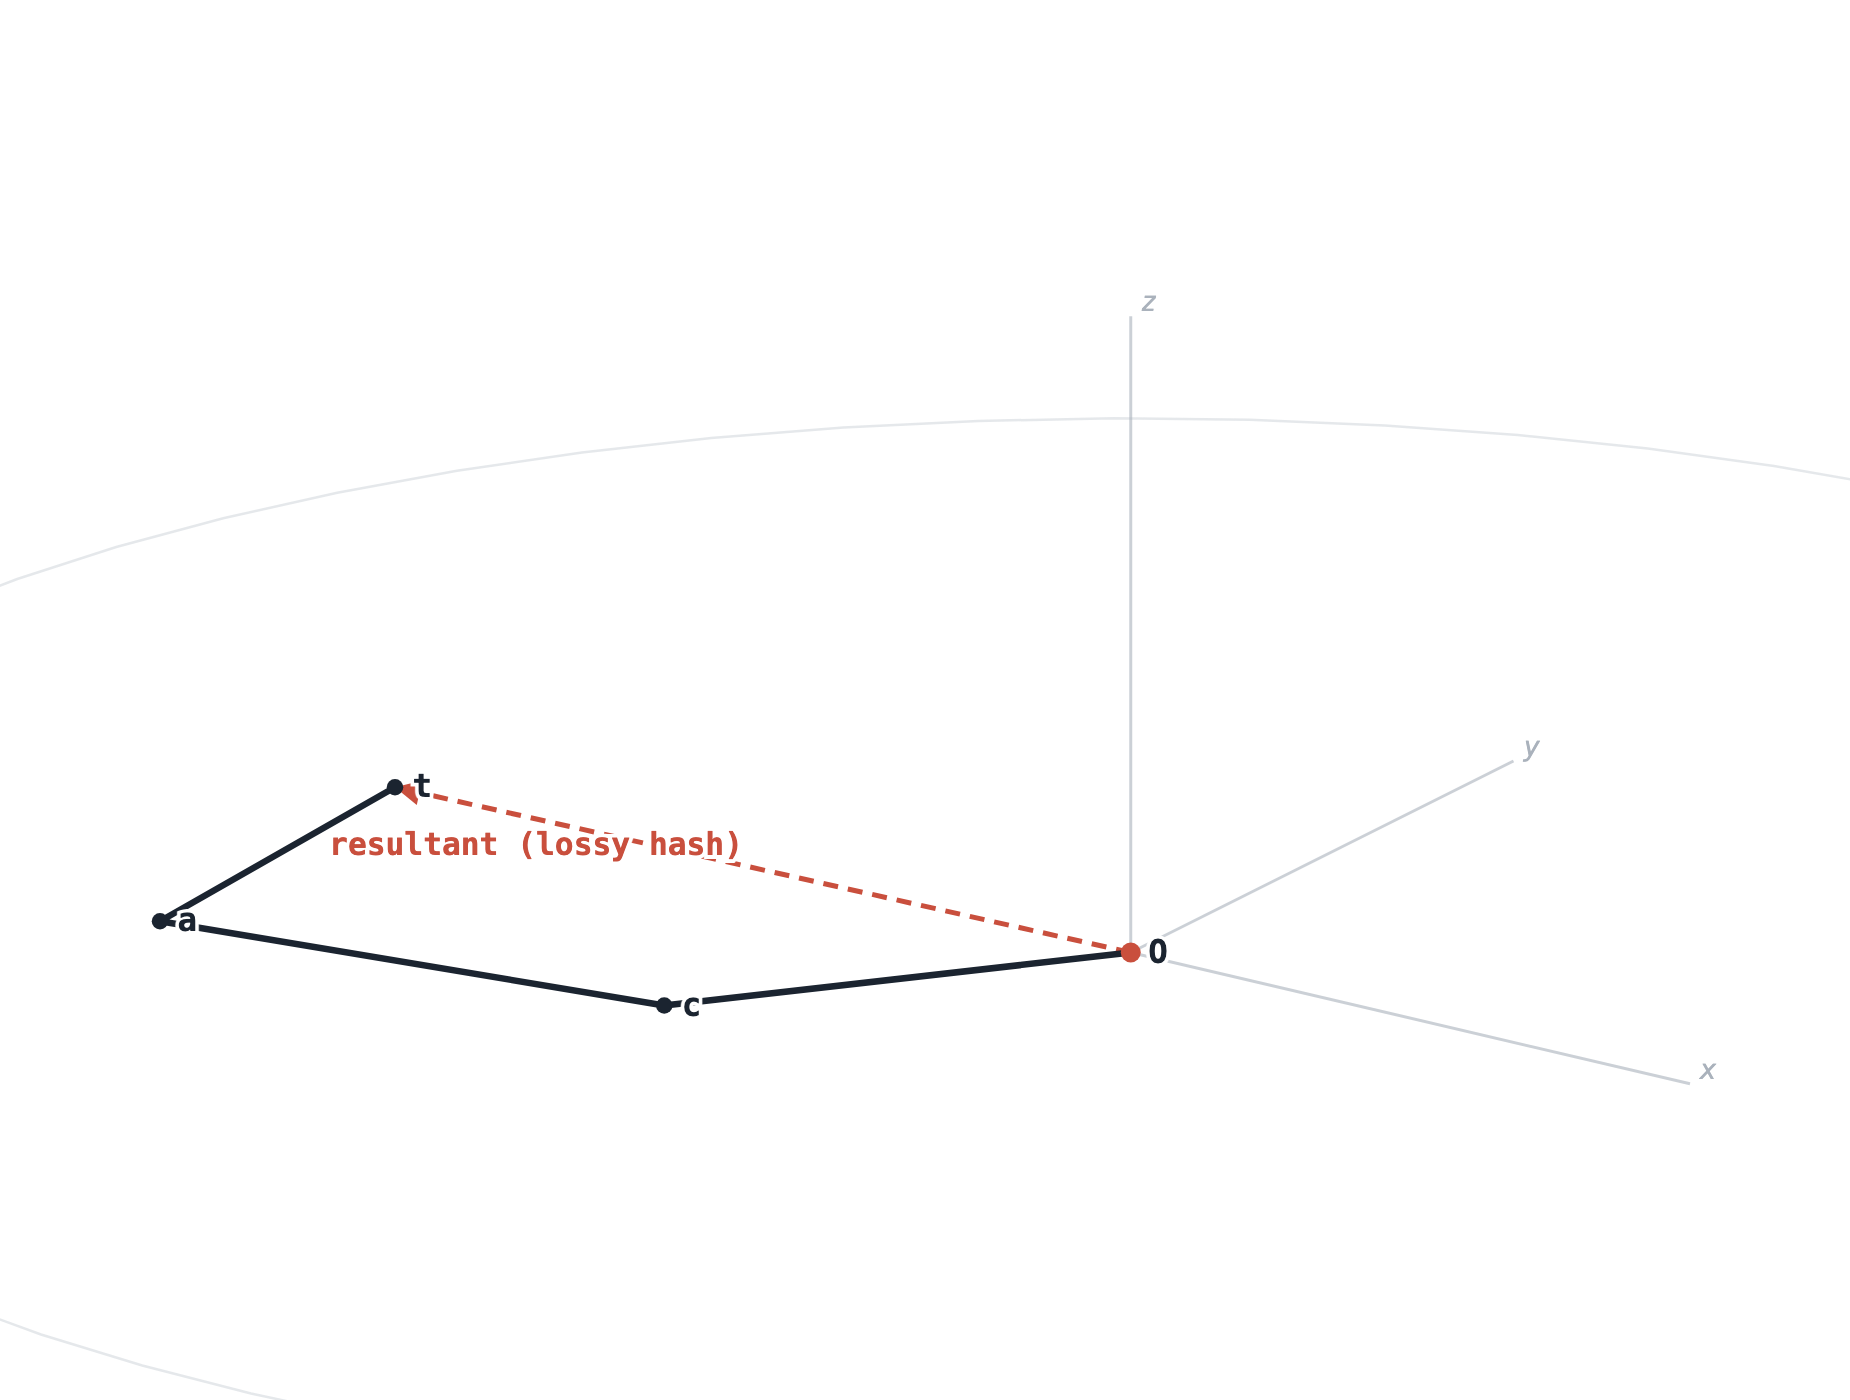
\includegraphics[width=0.82\linewidth]{figures/cat-resultant.png}
  \caption{The resultant of \texttt{cat}. The chain O$\to$c$\to$a$\to$t (black) and its
  resultant---the straight segment from the origin to the last node (red, dashed). The
  resultant is a lossy hash of the string: many strings share it, and it cannot be decoded
  back to the string.}
  \label{fig:resultant}
\end{figure}

Summing a chain's steps gives a single resultant vector, the straight segment from the origin
to the last node (the dashed line for \texttt{cat} in Figure~\ref{fig:resultant}). The sum is
lossy: a string of length $n$ has $90^n$ possibilities, while the resultant is three numbers
in a bounded region, so by the pigeonhole principle many strings share a resultant---already
$5.9$ billion strings of length five map into one bounded 3-vector. Its length alone, a single
number, collides far worse: infinitely many strings share it. The resultant is thus a
fingerprint or hash---useful for comparison and for low-collision matching of short
strings---but it cannot be decoded back to the string, because no information has been kept
that would reconstruct it. A hash is not a compression. Reversibility lives only in the full
chain (Section~\ref{sec:reversibility}); the resultant discards it.

\subsection{Phrases, dictionaries, and where savings come from}

A whole phrase can indeed be given a single vector, but only in one of two ways, and neither
escapes the entropy of the text. As a resultant it is the lossy hash above---not recoverable.
As a dictionary index, one code pointing to a stored phrase, it is ordinary dictionary coding:
the saving is real, since natural text is redundant and a good dictionary or tokenizer reaches
roughly $1$--$2$ bits per character, but the phrase still lives in the dictionary and the
total does not fall below the text's entropy. This saving is a property of the language's
redundancy, not of the geometry; the chain neither adds to it nor subtracts from it.

\subsection{What the representation costs}

The information a chain holds is (number of vectors) $\times$ (bits per vector), and both
factors are bounded---the bits per vector by precision, the count being exactly what must grow
to hold more content. For an encyclopedia of ten million characters, the entropy floor is
about $1$--$2$~MB once redundancy is removed (a purpose-built dictionary reaches
$\sim 2$~MB; the best compressors in existence reach $\sim 1$~MB), while the raw $90$-symbol
stream is $7.7$~MB. Stored as floating-point coordinates, the same chain occupies
$34$--$69$~MB---fifteen to thirty times the text, because each $6.5$-bit symbol becomes three
floating-point numbers. The right way to keep a chain is therefore to store the symbol
sequence and redraw the geometry on demand. None of the three hopes beats the entropy of the
input: packing coordinates finely buys a bounded one-time factor, the resultant loses the
string, and a dictionary merely relocates it. The value of the representation is legibility
and reversibility, not compression.

% =========================================================================
\section{Geometric fingerprints}\label{sec:fingerprints}

A deterministic, per-symbol map turns a string into a shape and a vocabulary into a family of
shapes. The shapes are not arbitrary: their structure records the structure of the words, and
reading it back is what makes the representation useful for matching
(Section~\ref{sec:applications}).

\subsection{Shared prefixes coincide}

In the cumulative encoding of Section~\ref{sec:encoding} the $k$-th step depends only on the
$k$-th symbol and on $k$, so two strings that begin alike begin identically---equal prefixes
give equal step vectors and equal partial chains. Drawn from a common origin, two strings
trace coincident curves up to the first position at which they differ, and fork there; the
chain is thus a visual diff of two strings aligned at their heads. In this mode, however, the
fingerprint is tied to the start of the text: because $\alpha$ accumulates from the first
symbol, the same word occurring later sits at higher elevations and traces a different shape.

\subsection{Position-invariant word shapes}

One change frees a word's shape from its position. Let $\alpha$ accumulate from the start of
each \emph{word} rather than the start of the text---reset at each delimiter, the $j$-th
letter of a word taking $\alpha=j\cdot\Delta$. A word's step vectors then depend only on its
spelling, so identical words trace congruent shapes wherever they occur, and the reset of
$\alpha$ marks each word boundary as a sawtooth in elevation, so segmentation is read from the
geometry itself. Within the length bound of Section~\ref{sec:reversibility} (a word of more
than $90\deg/\Delta$ letters re-enters the vertical) the map from word to shape is injective
up to translation: two words trace the same shape only if they are the same word.

\subsection{The vocabulary as a prefix tree}

Over a whole vocabulary these combine. Every word is a path from the origin; words sharing a
spelling prefix share the initial segment of their path and branch where they differ;
identical words coincide. A vocabulary therefore renders as a three-dimensional prefix
tree---a trie drawn in space (Figure~\ref{fig:prefixtree})---not by construction but as a
consequence of the deterministic map. Common beginnings bundle near the root, each fork marks
where spellings diverge, and the depth of a leaf is a word's length.

\subsection{Similarity, and its limits}

The geometry places similar words near one another: two words differing in a single letter
share every step but one and trace nearly-coincident shapes, and the distance between two
shapes grows with the edit distance of their spellings. This is the structure
Section~\ref{sec:applications} uses for approximate retrieval. Two limits are worth stating
plainly. The similarity is \emph{orthographic}, not semantic---\texttt{cat} and \texttt{cot}
are close, \texttt{cat} and \texttt{feline} are not---and it is \emph{ordered}: the shape
distinguishes anagrams (\texttt{cat} and \texttt{act} trace different paths), which is right
for identity but means the fingerprint is not invariant to permuting letters. A signature
invariant to rotation, scale, or meaning would need a different construction; we leave these
as open directions (Section~\ref{sec:limitations}).

% =========================================================================
\section{Related work}\label{sec:related}

The construction borrows several established ideas and applies them to a use they have not
been put to. We name the closest and mark what is, and is not, new here.

\paragraph{Internal coordinates (Z-matrix).} In computational chemistry a molecule is
specified in internal coordinates---each atom placed relative to earlier ones by a bond length
and one or two angles---rather than in absolute Cartesian coordinates~\cite{pulay1979}. This is
the same relative-step idea as ours: a length and angles positioning each unit with respect to
its predecessor. Protein backbones are described, and generated, from such coordinates one
residue after another, with no explicit index---order carried by the chain, exactly as here.
Of the precedents this is the closest; our contribution is not the internal-coordinate chain
but its use as a reversible, self-describing encoding of text, and the reading of the shapes
it produces.

\paragraph{Chain codes.} Freeman's chain code~\cite{freeman1961} represents a digitized curve
as a sequence of quantized step directions and is a staple of contour representation in image
processing; three-dimensional and differential variants exist. We share the ``curve as a
sequence of unit steps'' idea but invert the purpose: a chain code describes a given shape
compactly, whereas we manufacture a shape from symbols, binding a symbol's identity to a
step's direction.

\paragraph{Turtle graphics and L-systems.} Turtle geometry~\cite{abelson1981} defines a figure
as a stream of elementary move-and-turn instructions, and L-systems~\cite{lindenmayer1968,
abop1990} generate the branching forms of plants and fractals by rewriting strings into such
instruction streams. The string--geometry correspondence is the one we use to encode and
decode; our map is simply a fixed, invertible instruction per symbol rather than a generative
grammar.

\paragraph{Word-gesture keyboards.} Shape-writing systems (SHARK$^2$,
ShapeWriter)~\cite{zhai2003,kristensson2004,zhai2012} represent each word as a geometric
trajectory over a keyboard layout and recognize words by matching trajectories. The ``word as
a shape'' idea is theirs; the difference is that their shapes come from an arbitrary key
layout, whereas ours are a canonical, layout-independent function of spelling, and are
reversible.

Across these, the gap our work occupies is the use of an internal-coordinate chain as a
reversible, self-describing representation of text---and the prefix-tree visualization it
induces (Section~\ref{sec:fingerprints}), which we have not found described elsewhere.

% =========================================================================
\section{Applications}\label{sec:applications}

The representation does not compress (Section~\ref{sec:compression}), yet the same structure
that denies it compression makes it useful for distribution and retrieval. We sketch three
uses. Each is a systems benefit---a matter of where information sits and how fast it is
matched---not a claim of beating entropy.

\subsection{A shared geometric standard}

The map from symbols to vectors is a public convention, exactly as ASCII is a public
convention from bytes to characters: nothing about it needs to travel with a message. Raising
the convention from single characters to common words, phrases, and document templates---a
standard dictionary of stock chains---lets a document be represented by references into that
shared standard rather than by its full character stream. Like ASCII, the dictionary is
distributed once and shared by everyone; a document then carries only its references. This
removes, for free, the redundancy that is common to all documents---frequent words,
boilerplate, formatting. What it cannot remove is a document's own content: a public standard
cannot contain the specific text of every possible document, so a document's unique
information still travels, and by Section~\ref{sec:compression} that quantity is its entropy.
The shared dictionary is amortized across the corpus, and each document pays only for what is
unique to it---no more, and no less.

\subsection{Fingerprints for matching and deduplication}

Because the encoding is deterministic and shared prefixes trace shared paths
(Section~\ref{sec:fingerprints}), a word or phrase has a distinctive geometric signature, and
similar strings have similar signatures. This is what makes the shared dictionary practical:
to decide whether a phrase is already known, one compares signatures rather than raw text, and
near-matches surface as nearby shapes. For exact matching a signature is no better than a
hash; the geometric advantage is approximate retrieval---nearest-neighbour search over
signatures finds paraphrases and near-duplicates that an integer token id cannot. The lossy
resultant of Section~\ref{sec:compression} serves as a cheap first-pass key; the full chain
confirms an exact match.

\subsection{A compact working representation}

Tokenized against a shared standard, a document is a few hundred thousand vectors rather than
millions of characters. For operations that run over the token stream---comparison, search,
similarity---the smaller, richer stream can be faster to process and lighter to hold in
memory, provided the shared dictionary is a resident resource rather than reloaded per
document. These are the ordinary benefits of any tokenized representation; the geometry adds
the similarity structure of the previous subsection on top. None of this lowers the total
information in a corpus below its entropy. It changes only where that information sits---in the
shared standard---and what each document must carry: only its own.

% =========================================================================
\section{Limitations and outlook}\label{sec:limitations}

We collect the boundaries of the method, several already noted in place.

\paragraph{The pole.} A step at exactly $\alpha=90\deg$ points straight up and has no azimuth;
its character is unrecoverable regardless of context (Section~\ref{sec:reversibility}). The
loss is a single, detected position and is avoided by choosing $\Delta$ so that $k\cdot\Delta$
is never an odd multiple of $90\deg$, but the pole is an intrinsic singularity of the spherical
coordinate, not an artifact we can design away.

\paragraph{Bounded per-vector capacity.} A vector carries a fixed number of bits, capped by
precision---a few dozen at double precision, fewer in a noisy medium
(Section~\ref{sec:compression}). Refining the coordinates buys only logarithmic, one-time
gains. The representation grows with the content it holds; it does not compress, and stored as
coordinates it is larger than the text.

\paragraph{Orthographic, ordered similarity.} The fingerprint of
Section~\ref{sec:fingerprints} measures spelling, not meaning, and is sensitive to letter
order (it separates anagrams). It is not invariant to rotation, scale, or paraphrase.
Signatures with any of these invariances---a semantic one above all---would need a different
construction.

\paragraph{Alphabet.} The dial covers $90$ printable ASCII characters, the five least-frequent
dropped to keep the geometry clean; non-ASCII and multibyte text are not yet handled. A larger
or hierarchical dial would extend it, at some cost in angular resolution.

\paragraph{Length and segmentation.} The self-describing property and the position-invariant
word fingerprint hold only up to the length bound of Section~\ref{sec:reversibility}; long
words need a smaller $\Delta$, and the word-local mode relies on an explicit delimiter to reset
$\alpha$.

\paragraph{Outlook.} The most useful next steps are a signature invariant to position,
rotation, and scale for robust retrieval; a semantic rather than orthographic embedding; and an
evaluation of geometric approximate-matching (Section~\ref{sec:applications}) against standard
string- and token-based baselines on a real deduplication or retrieval task. This paper
establishes the representation and its properties; whether the geometric structure earns its
place against those baselines is the question we leave for that evaluation.

% =========================================================================
% NOTE: bibliographic details below are provisional and must be verified
% (exact pages, years, venues) before submission.
\begin{thebibliography}{9}
\bibitem{freeman1961} H.~Freeman. On the encoding of arbitrary geometric configurations.
  \emph{IRE Transactions on Electronic Computers}, EC-10(2):260--268, 1961.
\bibitem{abelson1981} H.~Abelson and A.~diSessa. \emph{Turtle Geometry: The Computer as a
  Medium for Exploring Mathematics}. MIT Press, 1981.
\bibitem{lindenmayer1968} A.~Lindenmayer. Mathematical models for cellular interactions in
  development, I \& II. \emph{Journal of Theoretical Biology}, 18:280--315, 1968.
\bibitem{abop1990} P.~Prusinkiewicz and A.~Lindenmayer. \emph{The Algorithmic Beauty of
  Plants}. Springer, 1990.
\bibitem{pulay1979} P.~Pulay, G.~Fogarasi, F.~Pang, and J.~E.~Boggs. Systematic ab initio
  gradient calculation of molecular geometries, force constants, and dipole moment
  derivatives. \emph{Journal of the American Chemical Society}, 101(10):2550--2560, 1979.
\bibitem{zhai2003} S.~Zhai and P.~O.~Kristensson. Shorthand writing on stylus keyboard. In
  \emph{Proc. CHI 2003}, 97--104.
\bibitem{kristensson2004} P.~O.~Kristensson and S.~Zhai. SHARK$^2$: a large vocabulary
  shorthand writing system for pen-based computers. In \emph{Proc. UIST 2004}, 43--52.
\bibitem{zhai2012} S.~Zhai and P.~O.~Kristensson. The word-gesture keyboard: reimagining
  keyboard interaction. \emph{Communications of the ACM}, 55(9):91--101, 2012.
\end{thebibliography}

\end{document}
